\section{Desarrollo de la propuesta}

\subsection{Comprensión y preparación de los datos}

En nuestro caso, el análisis comenzó una vez se nos fueron entregados los datos desde la Fundación Valle del Lili (FVL). Se nos dio un archivo del tipo ``Comma Separated Value'' (CSV) al que nos referiremos como ``dataset'' desde ahora. Nuestro análisis inicial se orientó principalmente a los objetivos específicos a y b. Con una descripción inicial del dataset encontramos como característica principal que no contiene nulos ni duplicados, razón por la que no se documenta limpieza alguna.

\begin{table}[H]
\centering
\caption{Métricas iniciales del dataset}
\begin{tabular}{|l|r|}
\hline
\textbf{Métrica} & \textbf{Valor} \\ \hline
Número de filas & 1324 \\ \hline
Número de columnas & 22 \\ \hline
Duplicados & 0 \\ \hline
Valores nulos totales & 0 \\ \hline
Ratio de desbalance & 0.4760 \\ \hline
\end{tabular}
\end{table}

A la par que recibimos los datos. Se nos fue entregado un diccionario de definiciones que describían la naturaleza de los datos (a excepción de su método de recolección). El diccionario contenía la siguiente información.

\begin{center}
\scriptsize 
\renewcommand{\arraystretch}{1.4} 
\begin{xltabular}{\textwidth}{|>{\raggedright\arraybackslash}p{5cm}|>{\raggedright\arraybackslash}X|>{\raggedright\arraybackslash}p{4cm}|}
\caption{Diccionario de variables del dataset} \label{tab:diccionario} \\
\hline
\textbf{Nombre de la variable} & \textbf{Definición} & \textbf{Tipo de variable} \\ \hline
\endfirsthead
\hline
\textbf{Nombre de la variable} & \textbf{Definición} & \textbf{Tipo de variable} \\ \hline
\endhead
\hline
\endfoot
\hline
\endlastfoot
EDAD & Edad del paciente & Cuantitativa continua (Entero) \\ \hline
GENERO & Género del paciente & Cuantitativa nominal (0:femenino, 1:masculino) \\ \hline
ACT\_FISICA\_METS & Paciente con actividad física & Cualitativa nominal (0: Inactiva, 1: Activa) \\ \hline
HB\_PREQX & Nivel de hemoglobina prequirúrgica & Cualitativa continua (Decimal), rango: 0.0 - 25.0 g/dL \\ \hline
HIPERTENSION & Alta presión en la sangre & Cualitativa nominal (0: Inactiva, 1: Activa) \\ \hline
DIABETES & Presencia de diabetes & Cualitativa nominal (0: Inactiva, 1: Activa) \\ \hline
ENFERMEDAD\_CORONARIA & Presencia de enfermedad coronaria & Cualitativa nominal (0: Inactiva, 1: Activa) \\ \hline
FALLA\_CARDIACA & Presencia de falla cardiaca & Cualitativa nominal (0: Inactiva, 1: Activa) \\ \hline
HIPOTIROIDISMO & Presencia de hipotiroidismo & Cualitativa nominal (0: Inactiva, 1: Activa) \\ \hline
ERC & Presencia de enfermedad renal crónica & Cualitativa nominal (0: Inactiva, 1: Activa) \\ \hline
INMUNOSUPRESION & Presencia de inmunosupresión & Cualitativa nominal (0: Inactiva, 1: Activa) \\ \hline
OBESIDAD & Presencia de obesidad & Cualitativa nominal (0: Inactiva, 1: Activa) \\ \hline
HIPERTENSION\_PULMONAR & Presencia de alta presión sanguínea en los pulmones & Cualitativa nominal (0: Inactiva, 1: Activa) \\ \hline
EPOC & Presencia de enfermedad pulmonar obstructiva crónica (COPD) & Cualitativa nominal (0: Inactiva, 1: Activa) \\ \hline
ASMA & Presencia de asma & Cualitativa nominal (0: Inactiva, 1: Activa) \\ \hline
ENF\_CEREBROVASCULAR & Presencia de enfermedad cerebrovascular & Cualitativa nominal (0: Inactiva, 1: Activa) \\ \hline
CANCER\_ACTIVO & Presencia de cualquier tipo de cáncer activo & Cualitativa nominal (0: Inactiva, 1: Activa) \\ \hline
TABAQUISMO & Tabaquismo & Cualitativa nominal (0: Inactiva, 1: Activa) \\ \hline
SANGRADO\_MAYOR & Si tuvo una pérdida excesiva de sangre en el momento de la cirugía & Cualitativa nominal (0: Inactiva, 1: Activa) \\ \hline
SHOCK & Presencia de shock hemorrágico hipovolémico después de la cirugía & Cualitativa nominal (0: Inactiva, 1: Activa) \\ \hline
MUERTE.1 & Muerte luego de la primera semana de cirugía & Cualitativa nominal (0: Inactiva, 1: Activa) \\ \hline
\end{xltabular}
\end{center}

Cada una de estas características estaban segmentadas por distintas categorías elegidas desde FVL.

\textbf{Características sociodemográficas:} EDAD, GENERO

\textbf{Características preoperativas:} ACT\_FISICA\_METS, HB\_PREQX

\textbf{Características en operación:} SANGRADO\_MAYOR

\textbf{Comorbilidades:} HIPERTENSION, DIABETES, ENFERMEDAD\_CORONARIA, FALLA\_CARDIACA, HIPOTIROIDISMO, ERC, INMUNOSUPRESION, OBESIDAD, HIPERTENSION\_PULMONAR, EPOC, ASMA, ENF\_CEREBROVASCULAR, CANCER\_ACTIVO, TABAQUISMO

\textbf{Características postoperativas:} SHOCK

\textbf{Resultados postoperativos:} MUERTE.1

\subsubsection{Variable objetivo}

Dado que shock es nuestra variable objetivo (VO), procedimos a analizar la distribución de las variables clínicas, comenzando por la VO. En la figura se observa un desbalance notable, con un 67.9\% de casos sin shock (0) y un 32.1\% de casos con shock (1). Esto indica una desproporción significativa entre ambas clases, el nivel de desbalanceo es de 2.1:1 calculándolo como siendo mucho más frecuentes los casos en los que no se presentó shock.

\begin{figure}[H]
\centering
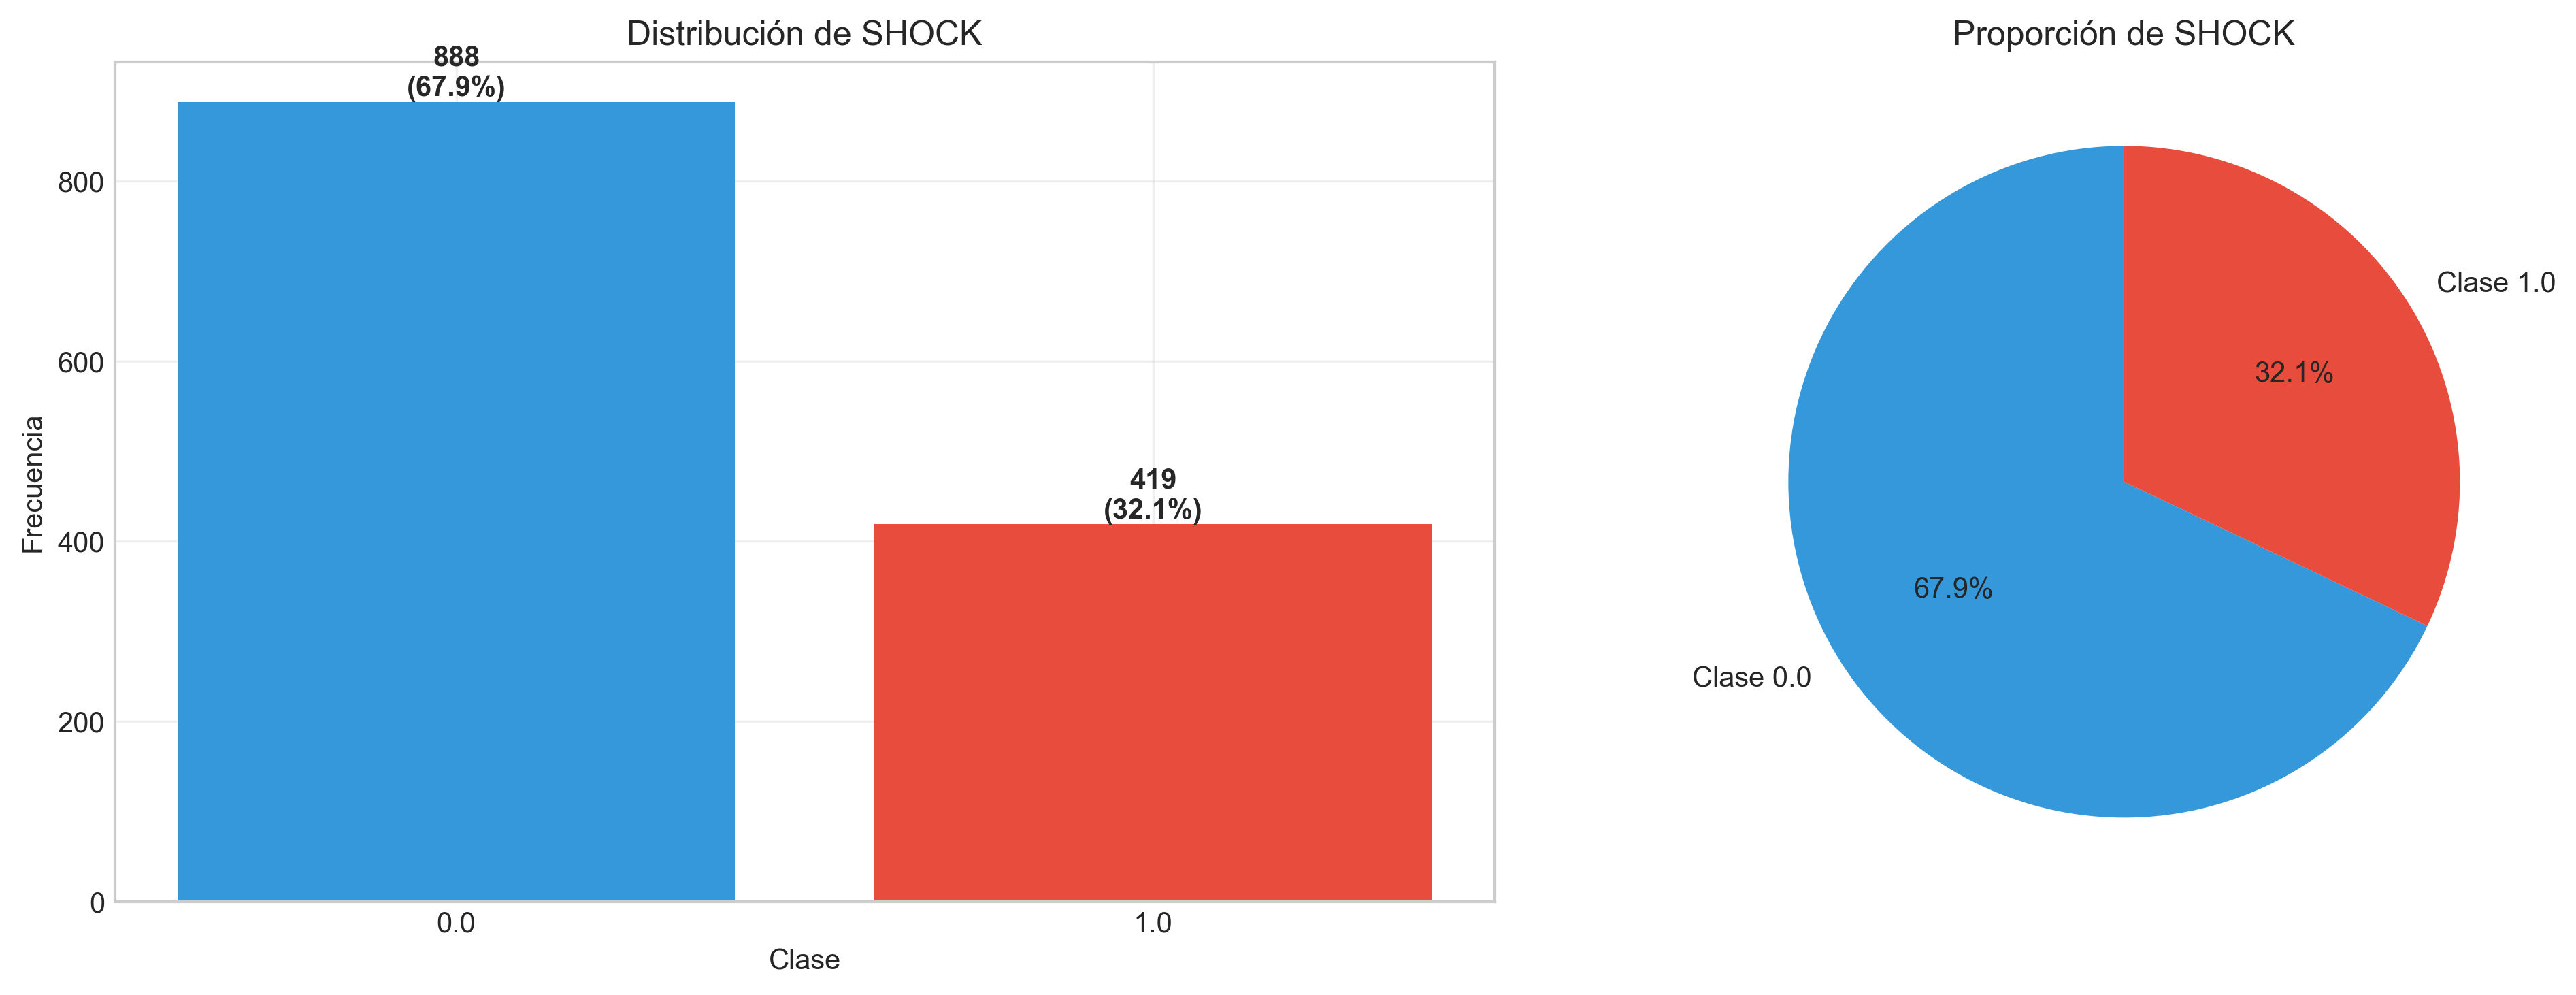
\includegraphics[width=\textwidth]{images/image002.png}
\caption{Variable objetivo - Shock}
\end{figure}

\subsubsection{Variables continuas}

Proseguimos con el análisis de Edad y HB\_PREQX. Lo que vemos son las distribuciones agrupadas por VO, donde las barras de color rosa corresponden a lo casos de shock y las barras de color café corresponden a los casos en los que no hubo shock. Vemos una distribución muy similar a una campana de Gauss para ambas variables, donde la mayoría de los casos se centran en las personas de 60 años para la variable de Edad. De igual forma, la variable HB\_PREQX tiene su mayor peso entre lo niveles 13 y 14. La forma en la que se medirá la relevancia contra la VO para las variables numéricas será con el estadístico de Cohen's d \cite{piasta2010}. Esta es una medida de tamaño del efecto que se utiliza para cuantificar la magnitud de la diferencia entre las medias de dos grupos, expresada en unidades de desviación estándar. Para ejecutarlo correctamente sobre la VO que es binaria, tomaríamos entonces la media de los casos en los que hubo shock y lo restamos con la media de las veces en las que no hubo, esto lo dividimos entre la desviación estándar agrupada para las medias de ambos grupos, formulando lo siguiente:

$$d = \frac{\bar{X}_{shock} - \bar{X}_{no\,shock}}{S_{pooled}}$$

A partir del coeficiente, se ha introducido una serie de rangos de interpretación formulados por el mismo autor del estadístico, los cuales son:

\begin{table}[H]
\centering
\caption{Interpretación del coeficiente de Cohen's d}
\begin{tabular}{|c|c|l|}
\hline
\textbf{Cota inferior (no inclusiva)} & \textbf{Cota superior (inclusiva)} & \textbf{Interpretación} \\ \hline
0 & 0.05 & Efecto muy pequeño \\ \hline
0.05 & 0.15 & Efecto pequeño \\ \hline
0.15 & 0.25 & Efecto mediano \\ \hline
0.25 & $+1$ & Efecto grande \\ \hline
\end{tabular}
\end{table}

Sin embargo, que el coeficiente de Cohens nos diga que es relevante no es suficiente si los datos que tenemos nos indican que realmente no hay suficientes datos para confirmar que es confiable. Para corregir esto usamos el valor P.

El valor P es otro estadístico que nos permite comprobar la hipótesis nula sobre un conjunto de datos \cite{wasserstein2016}. Formalmente se describe como:

Siendo nuestro caso, el que es ``No existe diferencia en las medias poblacionales de la variable numérica entre los dos grupos definidos por la VO.'', cada una de estas hipótesis siendo evaluada a un nivel de confianza de 0.05 para la aceptación de la nula. Así obteniendo tanto relevancia con la VO como confianza sobre la característica.

Con respecto a la descripción estadística de las variables numéricas, encontramos los siguientes datos:

\textbf{Edad:}
\begin{itemize}
    \item Promedio sin shock: 53.71 años
    \item Promedio con shock: 59.57 años
    \item Desviación estándar sin shock: 20.46 años
    \item Desviación estándar con shock: 18.79 años
    \item Mínimo: 1 año
    \item Máximo: 95 años
    \item Cohens-d: 0.294. Medianamente relevante.
    \item P\_value: 3.94E-07. Confiable.
\end{itemize}

\textbf{HB\_PREQX:}
\begin{itemize}
    \item Promedio: 12.926 g/dL
    \item Desviación estándar: 2.023 g/dL
    \item Mínimo: 5 g/dL
    \item Máximo: 19.0 g/dL
    \item Cohens-d: -0.0670. Nada relevante por sí mismo.
    \item P\_value: 0.262. Se rechaza la nula y se acepta que la cantidad de datos de la hemoglobina prequirúrgica por sí sola no es una característica que sea relevante para el entrenamiento.
\end{itemize}

\begin{figure}[H]
\centering
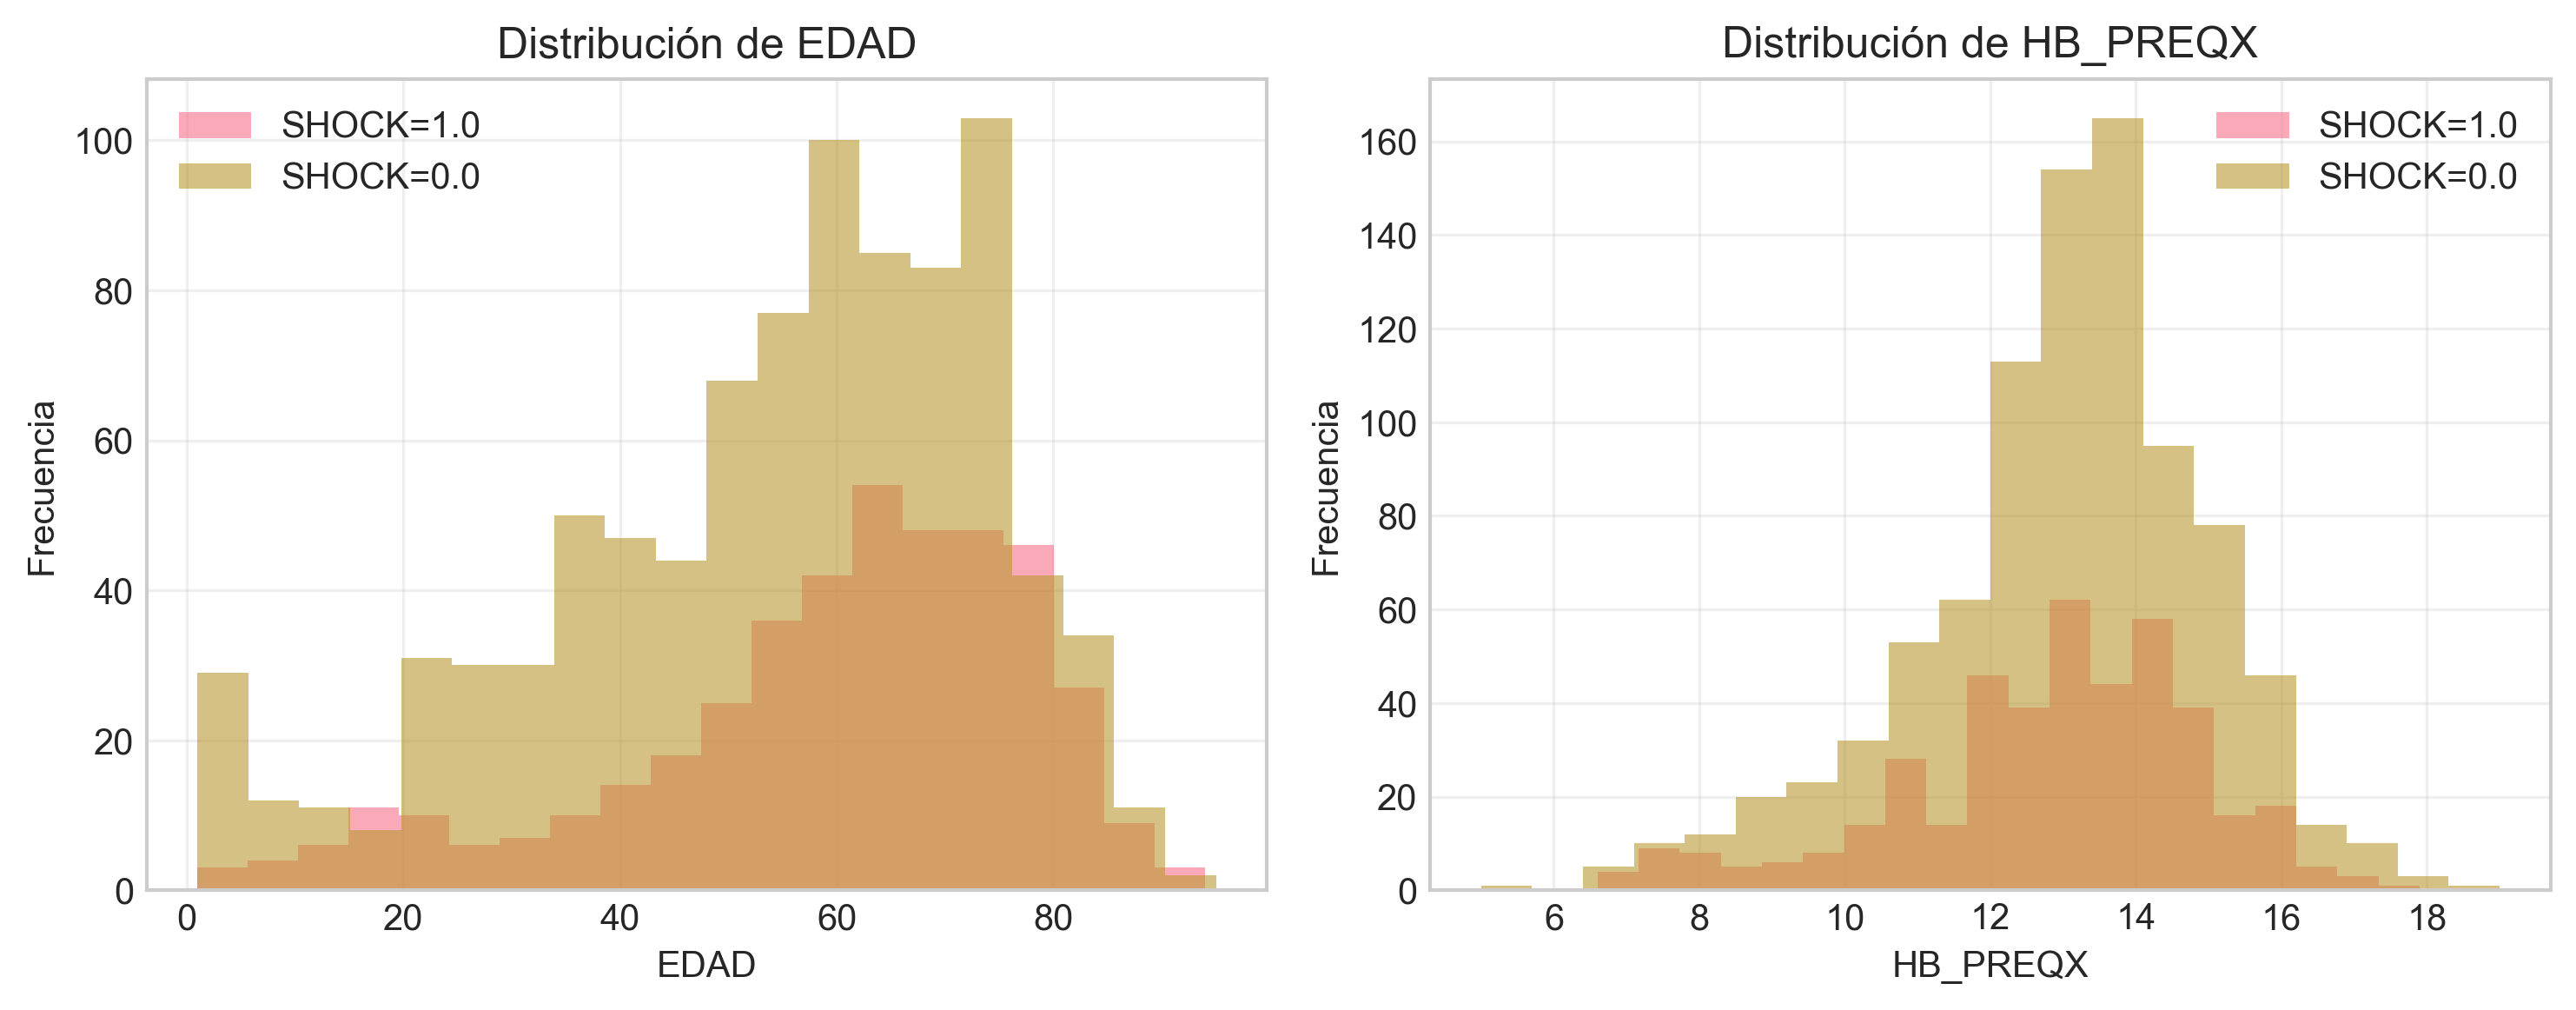
\includegraphics[width=\textwidth]{images/image007.png}
\caption{Interpretación de Cohen's d}
\end{figure}

\subsubsection{Variables booleanas}

La composición del resto del dataset eran datos categóricos booleanos, de estos solo se obtuvo su frecuencia y su relación con la VO. En el proceso describimos cada una de forma general, luego mostraremos nuestro procedimiento para descartar su influencia sobre la VO.

\textbf{GENERO:} Esta variable indica que hay una desproporción en los datos de hombres y mujeres en dataset, ya que vemos que los hombres (1) representan aproximadamente el 32\% del dataset, mientras que las mujeres ocupan aproximadamente el 68\% de este. Concluimos también que el shock afecta de igual forma tanto a hombres en la misma proporción.

\begin{figure}[H]
\centering
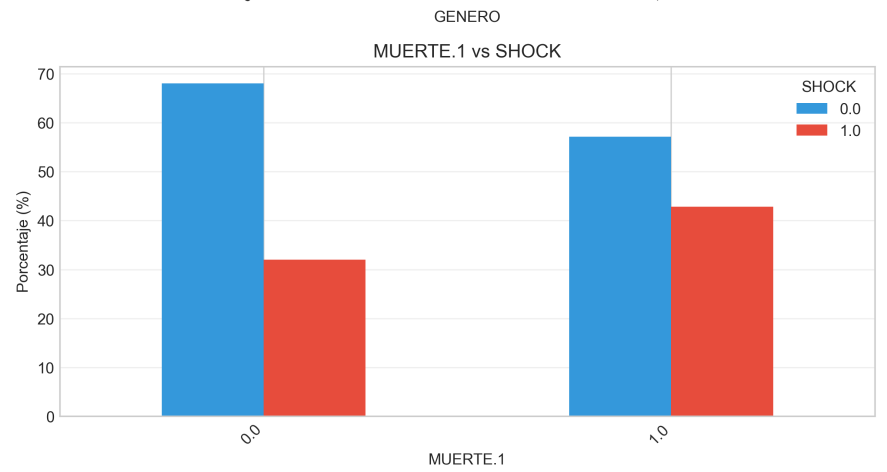
\includegraphics[width=\textwidth]{images/image010.png}
\caption{GENERO: Distribución por género}
\end{figure}

\textbf{ACT\_FISICA\_METS:} Se muestra una proporción similar al género en la actividad física, con un leve decremento cuando hay presencia de shock. Concluimos que el shock afecta en la misma medida a las personas que hacen deporte como a las que no.

\begin{figure}[H]
\centering
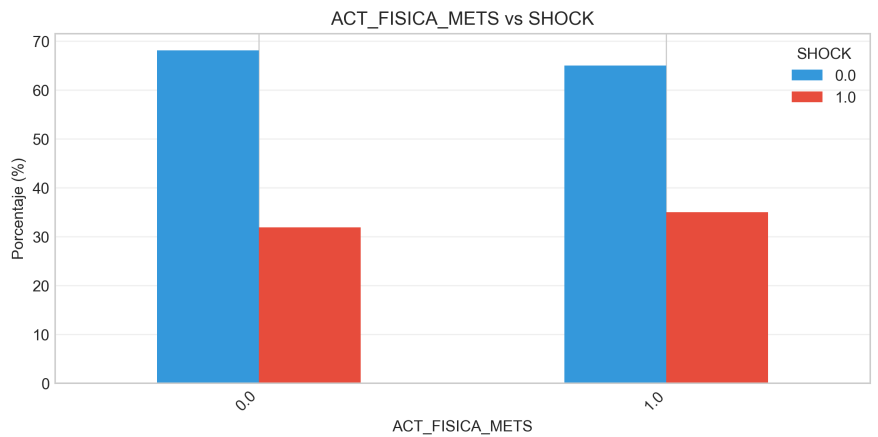
\includegraphics[width=\textwidth]{images/image009.png}
\caption{ACT\_FISICA\_METS: Actividad física}
\end{figure}

\textbf{Muerte:} Esta variable es postoperatoria es inservible cuando se trata de la predicción temprana del shock hipovolémico, por lo que no ha fue tomada en cuenta para el desarrollo temprano del modelo de IA. Sin embargo, esta variable será usada en posteriores análisis para la búsqueda de los mejores selectores. Vemos de igual modo que con respecto a la VO, que no todos los que murieron estuvieron relacionados con el shock.

\begin{figure}[H]
\centering
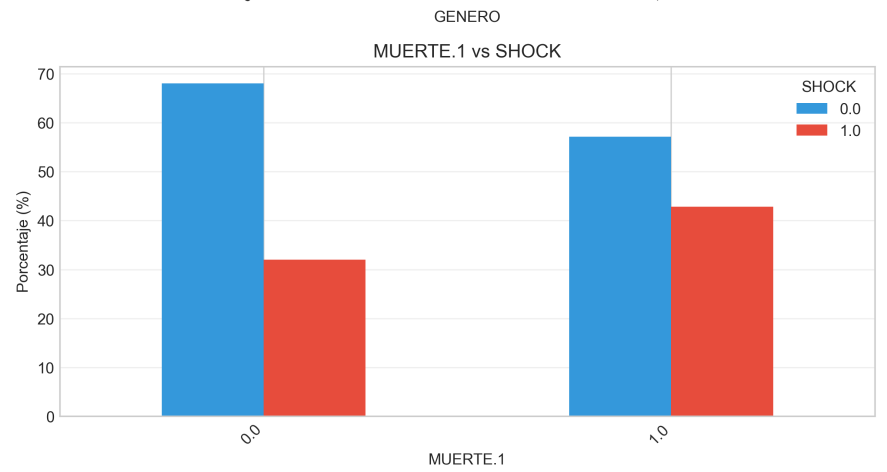
\includegraphics[width=\textwidth]{images/image010.png}
\caption{Muerte: Variable postoperatoria}
\end{figure}

\textbf{HIPERTENSION:} Con respecto al shock, la gráfica muestra que no hay diferencia entre las poblaciones que sufren o no hipertensión.

\begin{figure}[H]
\centering
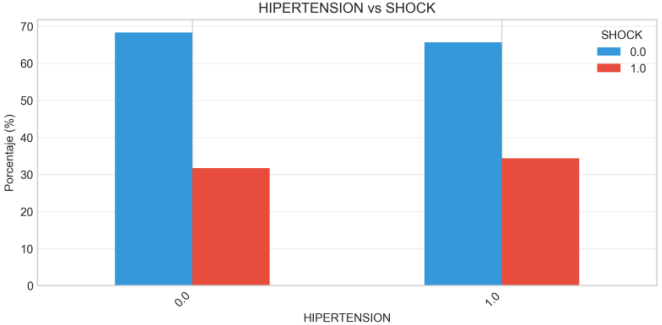
\includegraphics[width=\textwidth]{images/image011.png}
\caption{HIPERTENSION}
\end{figure}

\textbf{DIABETES:} En esta gráfica vemos que tampoco hay una mayor influencia sobre la VO.

\begin{figure}[H]
\centering
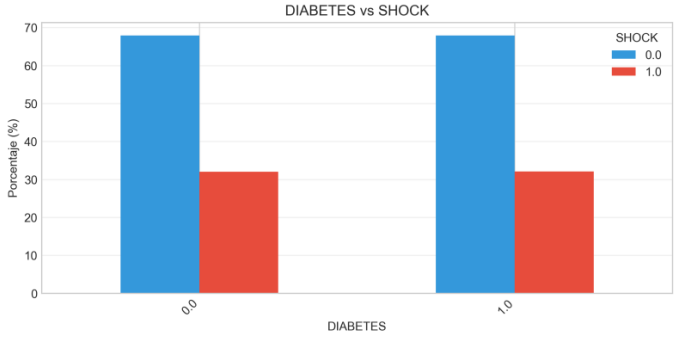
\includegraphics[width=\textwidth]{images/image012.png}
\caption{DIABETES}
\end{figure}

\textbf{ENFERMEDAD\_CORONARIA:} En este caso vemos una mayor influencia sobre la VO cuando se presenta esta comorbilidad, por lo que concluimos que podría ser un factor clave para el entrenamiento o las agregaciones.

\begin{figure}[H]
\centering
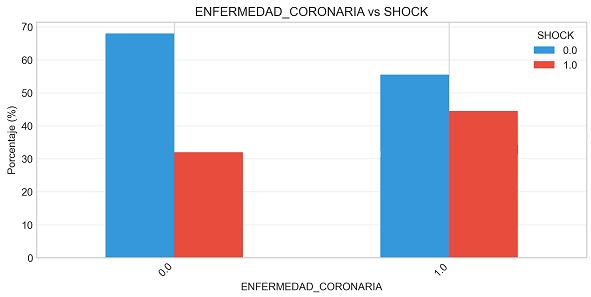
\includegraphics[width=\textwidth]{images/image013.png}
\caption{ENFERMEDAD\_CORONARIA}
\end{figure}

\textbf{FALLA\_CARDIACA:} Esta característica fue tratada como una que se ve afectada por el entorno controlado de los hospitales. Según los expertos de FVL este comportamiento resulta de que las personas con esta complicación son altamente monitoreadas, por lo que son menos propensas a sufrir un shock hipovolémico. Concluimos que la presencia de esta comorbilidad no influye en la VO.

\begin{figure}[H]
\centering
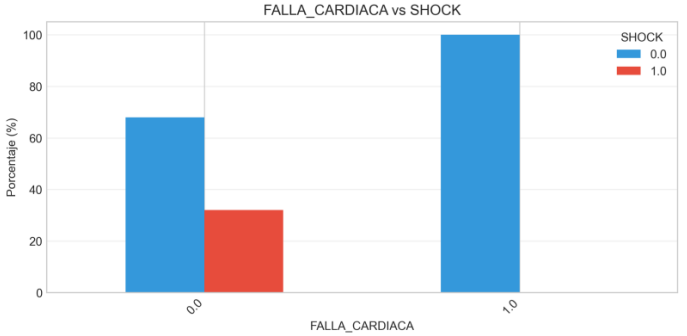
\includegraphics[width=\textwidth]{images/image014.png}
\caption{FALLA\_CARDIACA}
\end{figure}

\textbf{HIPOTIROIDISMO:} Vemos que no tiene mayor influencia en la VO.

\begin{figure}[H]
\centering
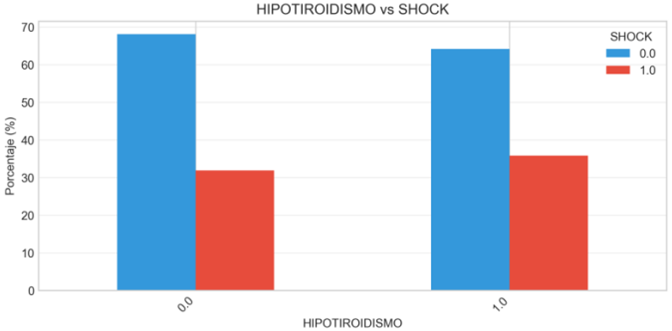
\includegraphics[width=\textwidth]{images/image015.png}
\caption{HIPOTIROIDISMO}
\end{figure}

\textbf{ERC:} Con esta variable podemos concluir que aquellas personas que presentan esta enfermedad son menos propensas a sufrir un shock hipovolémico, según los expertos de FVL tiene la misma explicación que con la falla cardiaca y el alto seguimiento del riesgo con las personas que presentan esta comorbilidad.

\begin{figure}[H]
\centering
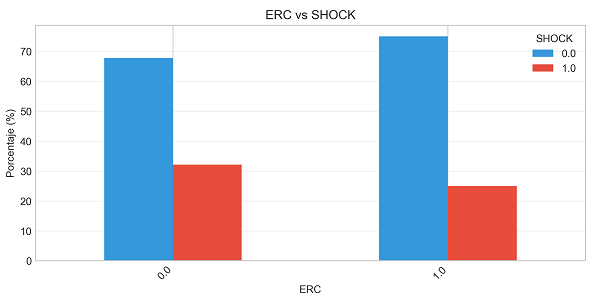
\includegraphics[width=\textwidth]{images/image016.png}
\caption{ERC}
\end{figure}

\textbf{OBESIDAD:} Vemos que la obesidad no influye de forma notoria sobre la VO.

\begin{figure}[H]
\centering
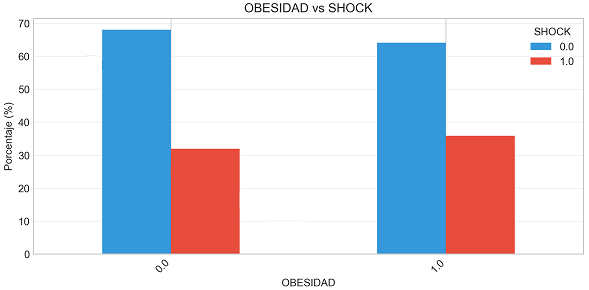
\includegraphics[width=\textwidth]{images/image017.png}
\caption{OBESIDAD}
\end{figure}

\textbf{HIPERTENSION\_PULMONAR:} En este caso, vemos que el poseer o no esta complicación afecta en gran medida el riesgo de shock.

\begin{figure}[H]
\centering
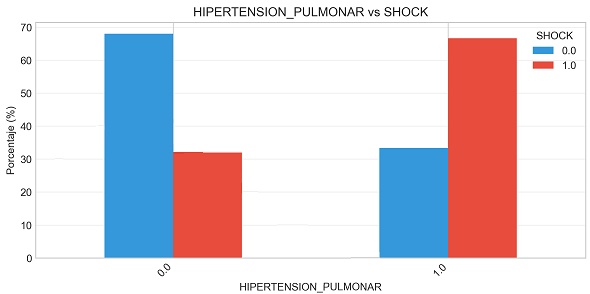
\includegraphics[width=\textwidth]{images/image018.png}
\caption{HIPERTENSION\_PULMONAR}
\end{figure}

\textbf{EPOC:} Aquí vemos que el poseer o no esta enfermedad no influye directamente en la VO.

\begin{figure}[H]
\centering
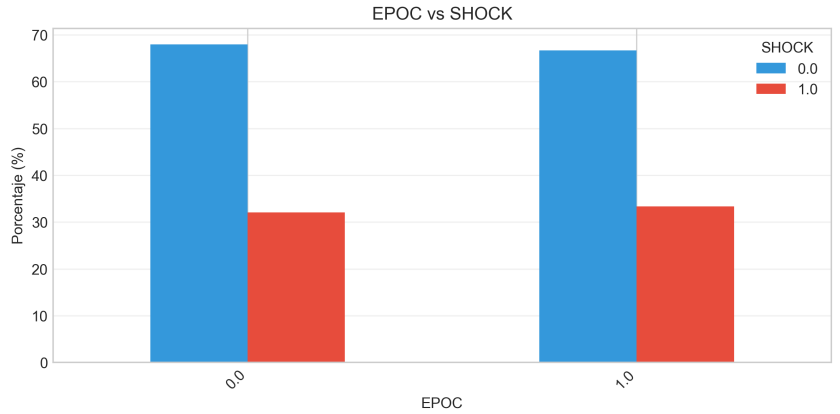
\includegraphics[width=\textwidth]{images/image019.png}
\caption{EPOC}
\end{figure}

\textbf{ASMA:} Vemos que no tiene una mayor incidencia sobre la VO.

\begin{figure}[H]
\centering
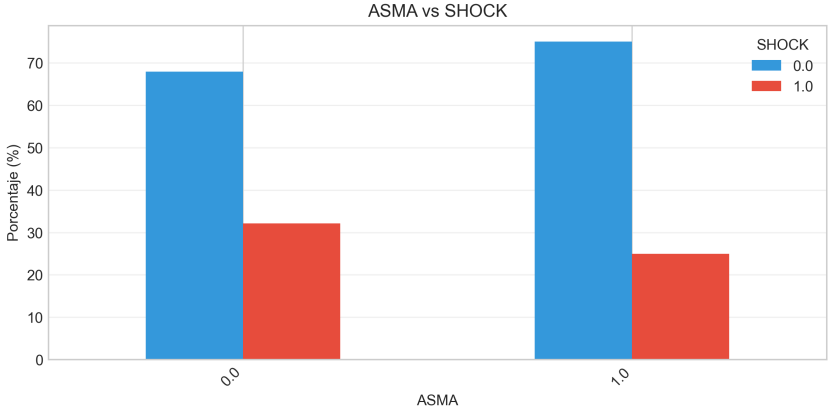
\includegraphics[width=\textwidth]{images/image020.png}
\caption{ASMA}
\end{figure}

\textbf{ENF\_CEREBROVASCULAR:} Vemos que no tiene mayor influencia sobre la VO.

\begin{figure}[H]
\centering
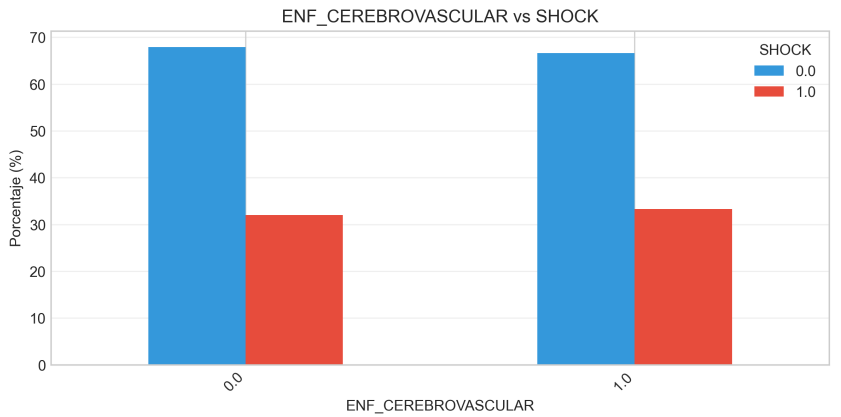
\includegraphics[width=\textwidth]{images/image021.png}
\caption{ENF\_CEREBROVASCULAR}
\end{figure}

\subsection{Discriminación inicial de la relevancia de las características sobre la VO}

Para poder tener una comprensión más detallada de que comorbilidades influían realmente sobre la VO usamos la matriz de coeficientes de Cramér's V \cite{allen2017}. Esta es una medida de asociación entre dos variables nominales que proporciona un valor entre 0 y 1 (inclusivo), donde 0 indica ausencia de asociación y 1 indica asociación perfecta. Este coeficiente se basa en la estadística de chi-cuadrado de Pearson y fue desarrollado por el estadístico sueco Harald Cramér.

La matriz de coeficientes de Cramér's V extiende este concepto calculando el coeficiente de Cramér's V para cada par de variables categóricas en un dataset, creando así una lista de correlación específica para variables categóricas, concepto ideal para el análisis de las comorbilidades booleanas. Al hacer la aplicación sobre el dataset se obtuvo la siguiente figura.

\begin{figure}[H]
\centering
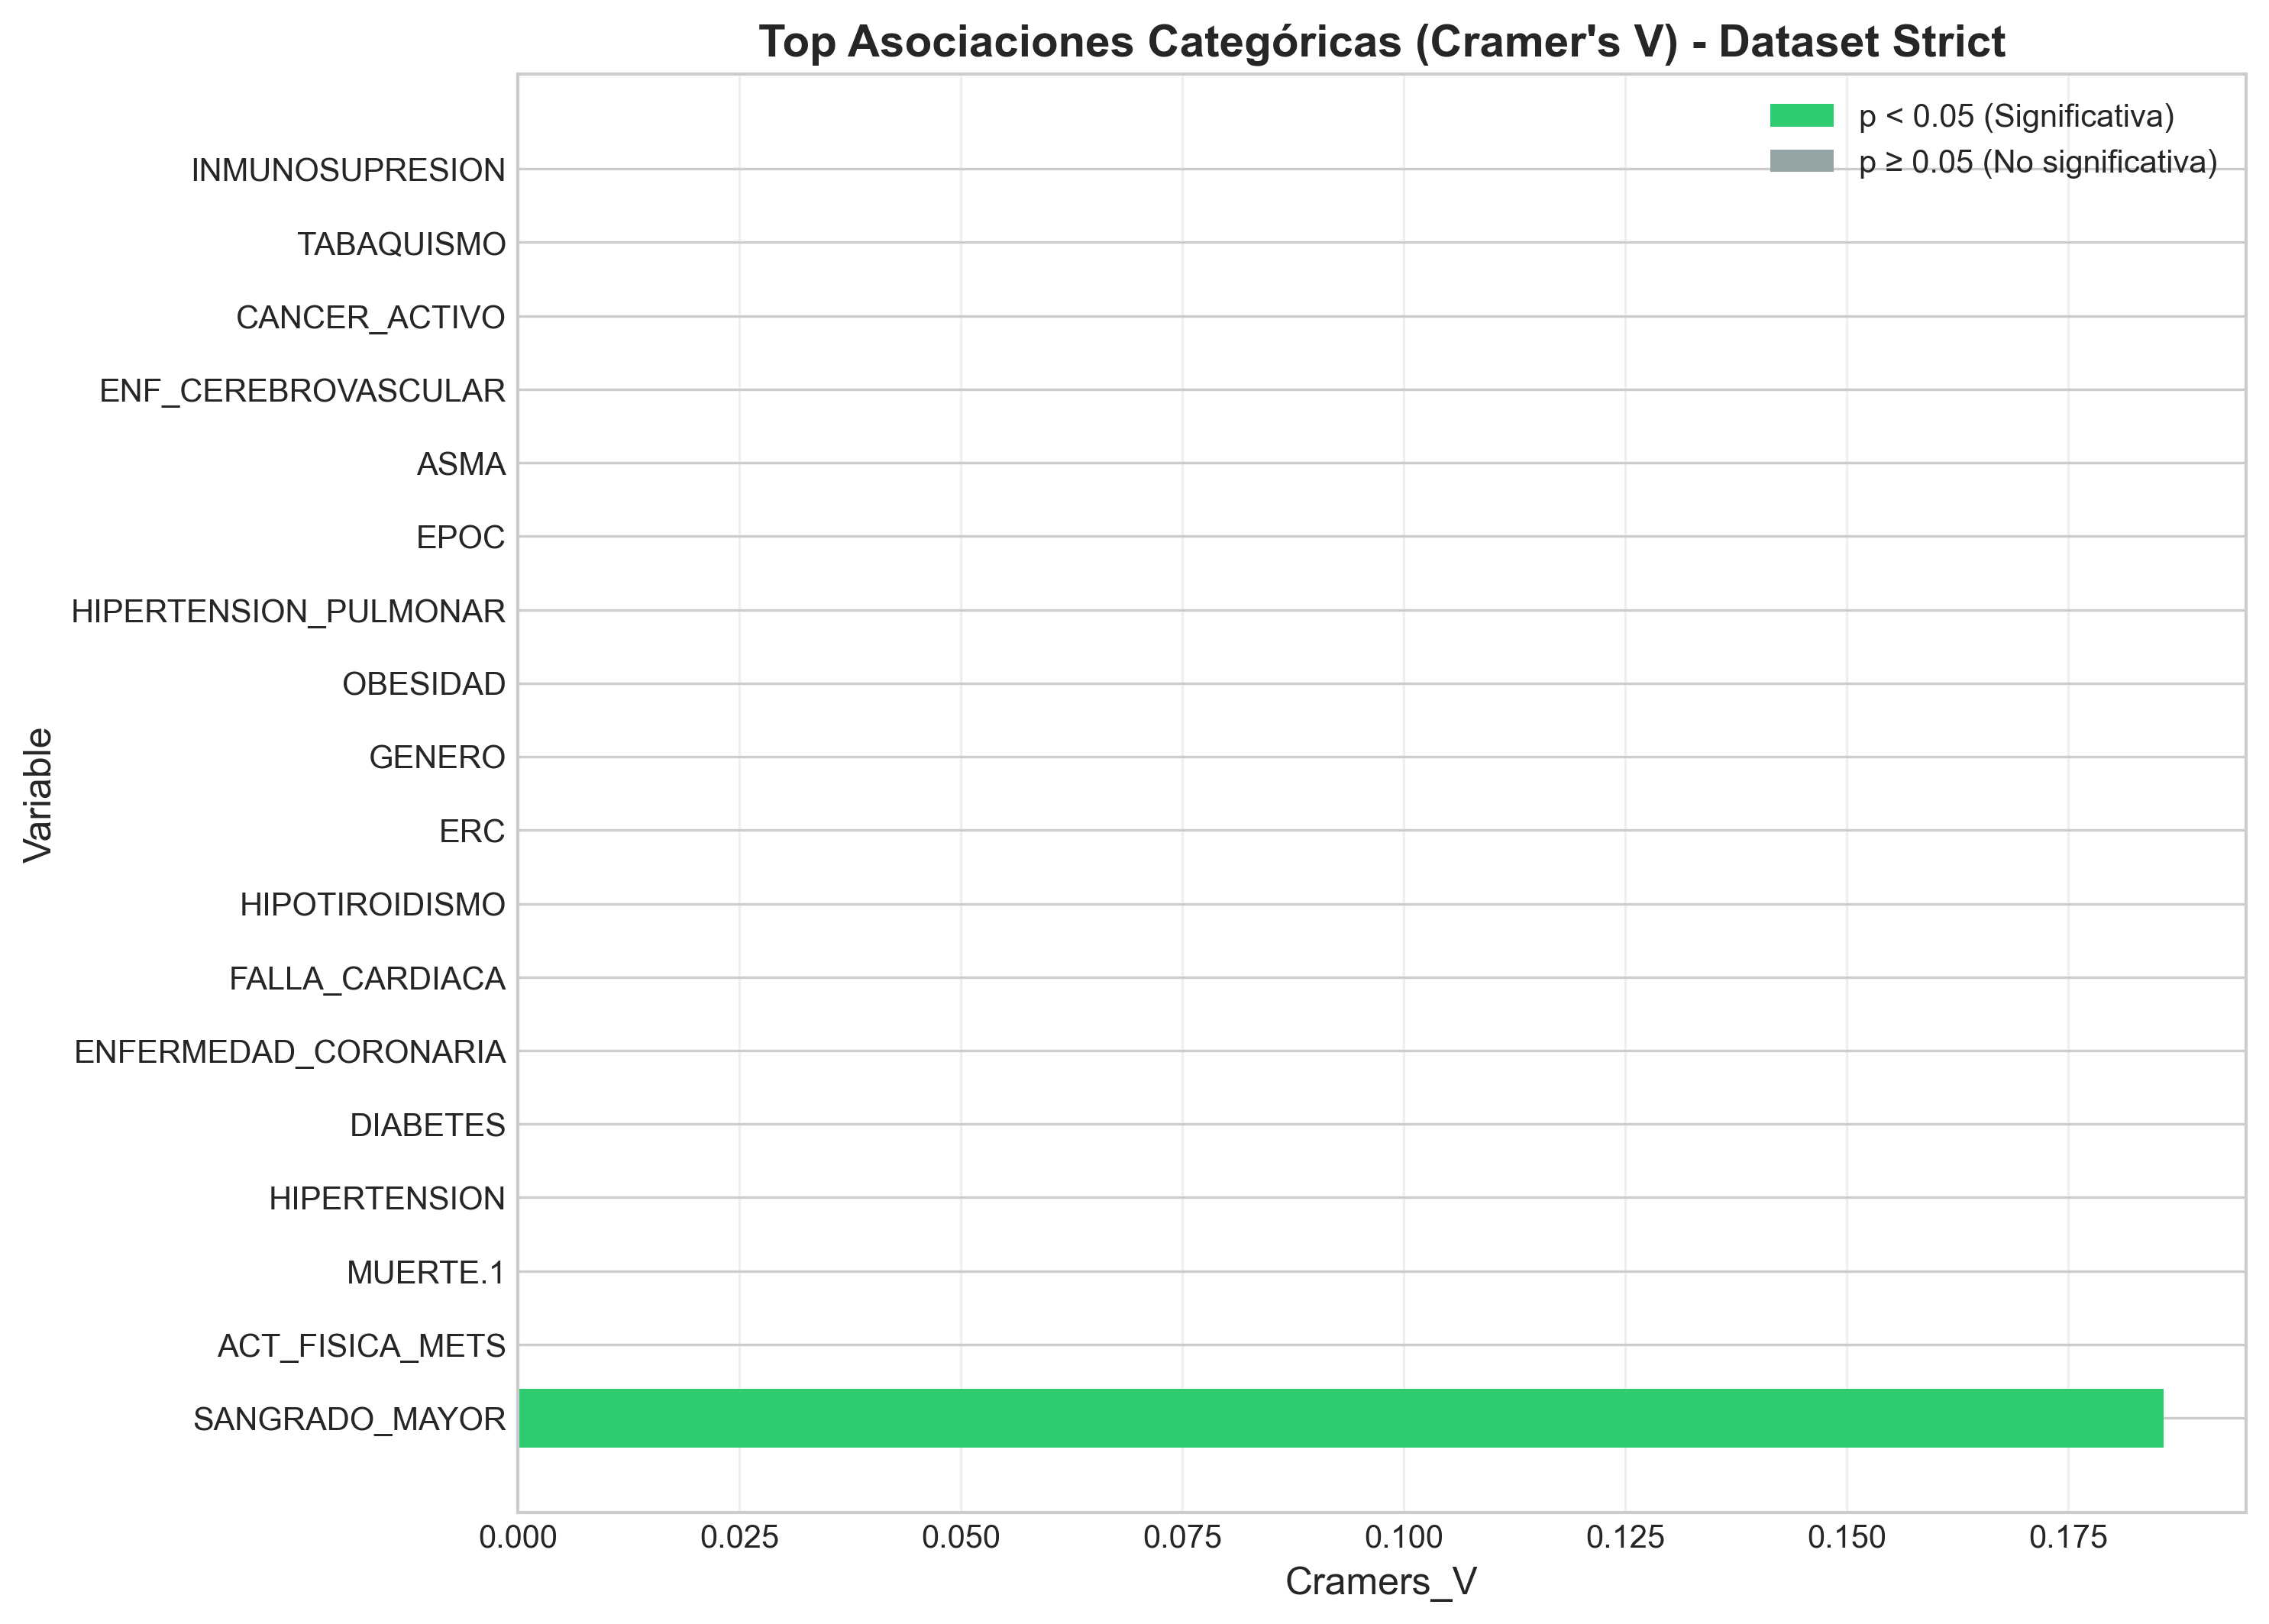
\includegraphics[width=\textwidth]{images/image022.png}
\caption{Matriz de Cramér's V}
\end{figure}
